\documentclass[10pt]{amsart}

\usepackage[top=2cm,bottom=1.5cm,left=2cm,right=2cm]{geometry}
\usepackage{amssymb}
\usepackage[shortlabels]{enumitem}
\usepackage{tikz}

\pagestyle{empty}

\theoremstyle{definition}
\newtheorem{problem}{Problem}

\definecolor{RoyalBlue}{cmyk}{1,0.50,0,0}
\newcommand{\demph}[1]{\textcolor{RoyalBlue}{\textbf{\textit{#1}}}}

% A framed space for students to write an answer. The argument is its height.
\newcommand{\answerbox}[1]{%
  \par\smallskip
  \noindent\fbox{%
    \parbox[t][#1][t]{%
      \dimexpr\linewidth-2\fboxsep-2\fboxrule\relax
    }{\strut}%
  }%
  \par\medskip
}

% A small answer box that can be used inside a displayed equation.

\newcommand{\inlineanswerbox}[1][3in]{%
  \ensuremath{%
    \vcenter{\hbox{%
        \fbox{\rule{0pt}{0.35in}\hspace{#1}}%
      }}%
  }%
}
% Format subsections as "Part 1: Title."
\makeatletter


\usepackage{titlesec}

\renewcommand{\thesubsection}{\arabic{subsection}}

\titleformat{\subsection}[block]{\normalfont\large\bfseries}{Part \thesubsection:}{0.5em}{}

\titlespacing*{\subsection}{0pt}{1em}{0.5em}
\makeatother

\tikzset{
  venn outline/.style={draw=black,very thick},
  venn fill/.style={fill=red!50},
  venn label/.style={font=\small}
}

\begin{document}
\thispagestyle{empty}

\section*{Worksheet 2: Set Theory}

\subsection{Set notation}

\begin{problem}[Reading a set]
  Let
  \begin{equation*}
    S=\{4,1,4,2,1,3\},
    \qquad
    T=\{3,2,4,1\}.
  \end{equation*}

  \begin{enumerate}[(a)]
    \item Rewrite $S$ without repetitions and find $|S|$.
    \begin{equation*}
      S = \inlineanswerbox \qquad |S| = \inlineanswerbox[.5in]
    \end{equation*}

    \item Decide whether each statement is true or false:
    \begin{center}
      \renewcommand{\arraystretch}{1.4}
      \begin{tabular}{l@{\qquad}cc}
        $2\in S$              & \textbf{T} & \textbf{F}\\
        $5\in S$              & \textbf{T} & \textbf{F}\\
        $\{1,2\}\subseteq S$  & \textbf{T} & \textbf{F}\\
        $\{1,2\}\in S$        & \textbf{T} & \textbf{F}
      \end{tabular}
    \end{center}

    \item Are $S$ and $T$ equal? Explain briefly.
    \vspace{1in}
  \end{enumerate}
\end{problem}

\begin{problem}[Set-builder notation]
  \begin{enumerate}[(a)]
    \item[]
    \item List the elements of $\{n\in\mathbb Z:-3\leq n\leq 3\}.$
    \vspace{1in}

    \item Describe the set $\{2,4,6,8,10,12,14,16,18,20\}$ using set-builder notation.
    \vspace{1in}

    \item List the elements of $P=\{(x,y):x\in\{1,2\}\text{ and }y\in\{a,b,c\}\}$.
    \vspace{2in}

    \item Find $|P|$.
  \end{enumerate}
\end{problem}
\newpage
\begin{problem}[Set operations]
  Let
  \begin{equation*}
    U=\{1,2,3,\ldots,12\},
    \qquad
    A=\{n\in U:n\text{ is even}\},
    \qquad
    B=\{n\in U:n\text{ is divisible by }3\}.
  \end{equation*}

  \begin{enumerate}[(a)]
    \item List the elements of $A$ and $B$.

    \begin{align*}
      A &=\inlineanswerbox\\[0.5em]
      B &=\inlineanswerbox\\[0.5em]
    \end{align*}


    \item Find each of the following sets:
    \begin{align*}
      A\cap B      &=\inlineanswerbox\\[0.5em]
      A\cup B      &=\inlineanswerbox\\[0.5em]
      A\setminus B &=\inlineanswerbox\\[0.5em]
      A^{c} &=\inlineanswerbox\\[0.5em]
      B^{c} &=\inlineanswerbox\\[0.5em]
    \end{align*}

    \item Is $A\subseteq B$? Explain.
    \vspace{1in}

    \item Are $A$ and $B$ disjoint? Explain.
    \vspace{1in}

  \end{enumerate}
\end{problem}

\newpage
\subsection{Two important set-theoretic results}

\begin{problem}[De Morgan's laws]
  Let $\Omega$ be a set. (The symbol $\Omega$ is called Omega, and is standard
  in probability). Let $A$ and $B$ be subset of $\Omega$.

  \begin{enumerate}[(a)]
    \item Shade $(A\cup B)^c$ in the first Venn diagram and
    $A^c\cap B^c$ in the second.

    \vspace{.5em}
    \begin{center}
      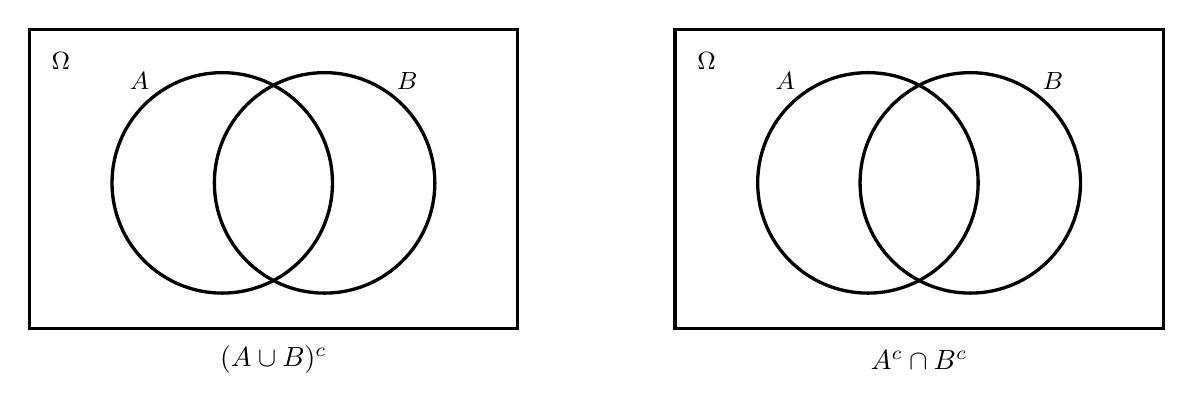
\begin{tikzpicture}
        \begin{scope}
          \draw[venn outline] (0,0) rectangle (6.2,3.8);
          \draw[venn outline] (2.45,1.85) circle (1.4);
          \draw[venn outline] (3.75,1.85) circle (1.4);
          \node[venn label] at (1.4,3.15) {$A$};
          \node[venn label] at (4.8,3.15) {$B$};
          \node[venn label] at (0.4,3.4) {$\Omega$};
          \node at (3.1,-0.4) {$(A\cup B)^c$};
        \end{scope}

        \begin{scope}[xshift=8.2cm]
          \draw[venn outline] (0,0) rectangle (6.2,3.8);
          \draw[venn outline] (2.45,1.85) circle (1.4);
          \draw[venn outline] (3.75,1.85) circle (1.4);
          \node[venn label] at (1.4,3.15) {$A$};
          \node[venn label] at (4.8,3.15) {$B$};
          \node[venn label] at (0.4,3.4) {$\Omega$};
          \node at (3.1,-0.4) {$A^c\cap B^c$};
        \end{scope}
      \end{tikzpicture}
    \end{center}
    \vspace{.5em}

    \item Are the shaded regions the same? Complete the identity
    \begin{equation*}
      (A\cup B)^c=\inlineanswerbox[1in]
    \end{equation*}
    % \item Complete the related identity 
    % \begin{equation*}
    %   (A\cap B)^c=\inlineanswerbox[1in]
    % \end{equation*}
  \end{enumerate}
\end{problem}


\begin{problem}[The inclusion--exclusion formula]
  The \demph{inclusion--exclusion formula} states that if $A$ and $B$ are
  finite sets, then
  \begin{equation*}
    |A\cup B|=|A|+|B|-|A\cap B|.
  \end{equation*}

  Explain why this identity holds using pictures.

  \vspace{3in}
\end{problem}

\subsection{Connection to probability theory}

\begin{problem}[Dice sets]
  Suppose we roll two dice. We represent the outcome by an ordered pair
  $(x,y)$, where $x$ is the result of the first dice and $y$ is the result of
  the second. The set of all possible outcomes is
  \begin{equation*}
    S=\{(x,y):x,y\in\{1,2,3,4,5,6\}\}.
  \end{equation*}

  \begin{enumerate}[(a)]
    \item How many elements does $S$ contain? Explain how you can count
    them without listing every element.
    \vspace{.9in}

    \item Let $B$ be the set of outcomes for which the sum of the two dice is $7$.
    Describe $B$ in set-builder notation, and then list its elements.
    \vspace{.9in}

    \item Let $C$ be the set of outcomes for which the two dice roll the same
    number. Describe $C$ in set-builder notation, and then list its elements.
    \vspace{.9in}

    \item Describe the following three sets in words. What events do they represent?
    \begin{equation*}
      D=\{(x,y)\in\Omega:x>y\},
      \qquad
      E=\{(x,y)\in\Omega:x=6\text{ or }y=6\},
      \qquad
      F=\{(1,1)\}.
    \end{equation*}
    \vspace{1.3in}

    \item In probability we use the word ``event'' rather than ``set''.
    Describe the following events in set-builder notation:
    \begin{enumerate}[(i)]
      \item The event that the dice add up to at least $10$.
      \vspace{.8in}
      \item The event that at least one dice shows an even number.
      \vspace{.8in}
    \end{enumerate}


    \item List the elements of the following sets
    \begin{align*}
      B\cap E &= \inlineanswerbox\\
      C\backslash E &= \inlineanswerbox
    \end{align*}
    \item Compute the following probabilities:
    \begin{alignat*}{2}
      \mathbb P(D) &={}\inlineanswerbox[2in] &\qquad \mathbb P(E) &={}\inlineanswerbox[2in] \\
      \mathbb P(F) &={}\inlineanswerbox[2in] &\qquad \mathbb P(B\cap E) &={}\inlineanswerbox[2in]
    \end{alignat*}
  \end{enumerate}
\end{problem}

\end{document}
